\documentclass[12pt, t]{beamer}

%------------------------------------------------------------------------------
% configuration
%------------------------------------------------------------------------------
\RequirePackage{etex}
\usepackage{currfile-abspath}
\usepackage{../../themes/dbt}
\usepackage{catchfilebetweentags}

\setbeameroption{hide notes}
\setbeamertemplate{caption}{\raggedright\insertcaption\par}

\graphicspath{{images/}}
\getmainfile
\getabspath{\themainfile}
\let\mainabsdir\theabsdir
\let\mainabspath\theabspath

\newcommand{\insertcode}[2]{\lstinputlisting[label=samplecode, basicstyle=#1]{\mainabsdir/code/#2}}
\newcommand{\bi}{\begin{itemize}}
\newcommand{\ei}{\end{itemize}}
\newcommand{\ig}{\includegraphics}
\newcommand{\myhref}[1]{\href{#1}{\tt \scriptsize #1}}
\newcommand{\incnote}[1]{\note{\ExecuteMetaData[notes.tex]{#1}}}
\newcommand{\src}[2]{\vspace{-10pt}\caption{\href{#1}{\centering \tt \tiny [#2]}}}


%------------------------------------------------------------------------------
% title
%------------------------------------------------------------------------------
%------------------------------------------------------------------------------
% title
%------------------------------------------------------------------------------
% slide
\title{Systèmes d'exploitation pour l'embarqué}
\subtitle{UV 5.2 - Exécution et Concurrence}

\author{\href{}{Paul Blottière}}
\institute{
    \href{http://www.ensta-bretagne.fr/}{ENSTA Bretagne} \\[2pt]
    \href{}{\tt \scriptsize 2018 / 2019}
}
\date{
    \href{https://github.com/pblottiere}{\tt \scriptsize https://github.com/pblottiere} \\[2pt]
    %\href{blottiere.paul@gmail.com}{\tt \scriptsize blottiere.paul@gmail.com}
}

% info
\begin{document}

{
\setbeamertemplate{footline}{} % no page number here
\frame{
    \titlepage
} }

%------------------------------------------------------------------------------
% amélioration continue
%------------------------------------------------------------------------------
\begin{frame}{Amélioration continue}
    \subt{Contributions}
    \vspace{12pt}

    \begin{center}
    
\includegraphics[scale=0.7]{github.png}
    \end{center}

    \bi
    \itemsep12pt
    \item Dépôt du cours : \href{https://github.com/pblottiere/embsys}{\tt \scriptsize https://github.com/pblottiere/embsys}
    \item Souhaits d'amélioration, erreurs, idées de TP, ... : ouverture d'Issues
    \item Apports de corrections : Pull Request
    \ei
\end{frame}




%<**lecture_content>
%------------------------------------------------------------------------------
% lecture
%------------------------------------------------------------------------------
\begin{frame}[plain,c]
    \centering
    \huge\textcolor{title}{Mémoire et système de fichiers}
\end{frame}

%------------------------------------------------------------------------------
% plan
%------------------------------------------------------------------------------
\begin{frame}{Plan}
    \subt{}
    \vspace{15pt}

    \begin{enumerate}
        \itemsep12pt
        \item Généralités
        \item RAM
        \item ROM
        \item Flash
        \item Systèmes de fichiers
        \item Les outils sous Linux
    \end{enumerate}

    \note {
    }
\end{frame}

%------------------------------------------------------------------------------
% gen1
%------------------------------------------------------------------------------
\begin{frame}{Généralités (1)}
    \subt{Caractéristiques}

    \vspace{15pt}
    Il existe deux familles de mémoire :
    \bi
    \itemsep8pt
    \item mémoire vive ou RAM (Random Access Memory)
    \item mémoire morte ou ROM (Read Only Memory)
    \ei

    \onslide<2->
    {
        \vspace{15pt}
        Chacune de ces familles peut être caractérisée par :
        \bi
        \itemsep10pt
        \item la capacité
        \item la durée de vie
        \item le temps d'accès
        \item le coût
        \ei
    }

\end{frame}

%------------------------------------------------------------------------------
% gen2
%------------------------------------------------------------------------------
\begin{frame}{Généralités (2)}
    \subt{Arbre généalogique}

    \begin{figure}
        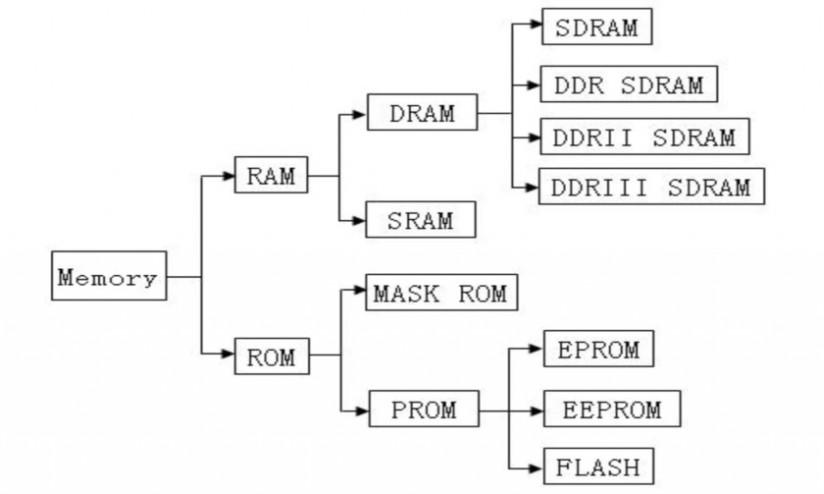
\includegraphics[scale=0.5]{tree.jpg}
    \end{figure}
\end{frame}

%------------------------------------------------------------------------------
% ram1
%------------------------------------------------------------------------------
\begin{frame}{RAM (2)}
    \subt{Définition}

    \vspace{8pt}
    Mémoire volatile : perte des données en cas de coupure de l'alimentation du
    périphérique.

    \onslide<2->
    {
        \vspace{8pt}
        Plusieurs types :
        \bi
        \itemsep6pt
        \item {\textbf{DRAM}} (Dynamic RAM) : les transistors (déchargés ou
            chargés => bit 0 ou 1) doivent être periodiquement rafraîchit
            (charge toutes les N ms) pour compenser les fuites.
        \item {\textbf{SRAM}} (Static RAM) : comme la DRAM mais pas besoin de
              rafraîchissement
          \item {\textbf{SDRAM}} (Synchronous DRAM) : synchronisation avec
              l'horloge du CPU
          \item {\textbf{DDR SDRAM}} (Double Data Rate SDRAM) : sur tous les
              PC standards. Grande bande passante.
        \item ...
        \ei
    }
\end{frame}

%------------------------------------------------------------------------------
% ram2
%------------------------------------------------------------------------------
\begin{frame}{RAM (2)}
    \subt{DDR en images}

    \begin{figure}
        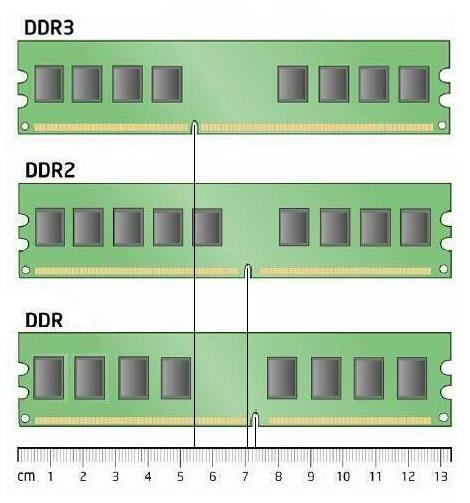
\includegraphics[scale=0.35]{ddr-compare.jpg}
    \end{figure}

\end{frame}

%------------------------------------------------------------------------------
% rom1
%------------------------------------------------------------------------------
\begin{frame}{ROM (1)}
    \subt{Caractéristiques}

    \vspace{8pt}
    Mémoire véritable : données persistantes même après coupure de
    l'alimentation.

    \onslide<2->
    {
        \vspace{8pt}
        Plusieurs types :
        \bi
        \itemsep8pt
        \item {\textbf{ROM}} (Read Only Memory) : programmée une seule fois
              lors de sa fabrication.
        \item {\textbf{PROM}} (Programmable ROM) : peut être programmée une fois
            par un utilisateur par un {\textit{programmateur}}. Obsolète.
          \item {\textbf{EPROM}} (Erasable PROM) : effaçable par UV et
              reprogrammable.
          \item {\textbf{EEPROM}} (Eletrically EPROM) : effaçable par faible
              tension et à la volée.
        \ei
    }
\end{frame}

%------------------------------------------------------------------------------
% rom2
%------------------------------------------------------------------------------
\begin{frame}{ROM (2)}
    \subt{En images}

    \begin{figure}
        \vspace{35pt}
        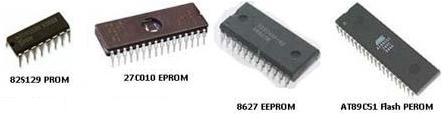
\includegraphics[scale=0.8]{list_rom.jpg}
    \end{figure}

\end{frame}

%------------------------------------------------------------------------------
% rom3
%------------------------------------------------------------------------------
\begin{frame}{ROM (3)}
    \subt{CHS}

    \vspace{6pt}
    {\textbf{Cyinder/Head/Sector}} : géométrie d'un disque.

    \vspace{6pt}
    {\textbf{Disque dur}} : plusieurs plateaux.

    \vspace{6pt}
    {\textbf{Plateau}} : plusieurs pistes circulaires.

    \vspace{6pt}
    {\textbf{Piste}} : plusieurs secteurs (1 -> S).

    \vspace{6pt}
    {\textbf{Cylindre}} : union des mêmes pistes de tous les plateaux (0 -> N-1).

    \vspace{6pt}
    {\textbf{Tête d'écriture/lecture}} : 2 par plateau (0 -> N-1).

    \onslide<2->
    {
        \vspace{6pt}
        \begin{figure}
            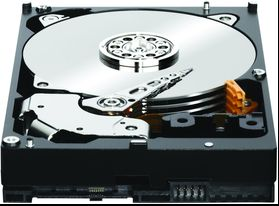
\includegraphics[scale=0.8]{disque_dur_autopsie.jpg}
        \end{figure}
    }
\end{frame}

%------------------------------------------------------------------------------
% rom4
%------------------------------------------------------------------------------
\begin{frame}{ROM (4)}
    \subt{Autopsie}

    \vspace{15pt}
    \begin{figure}
        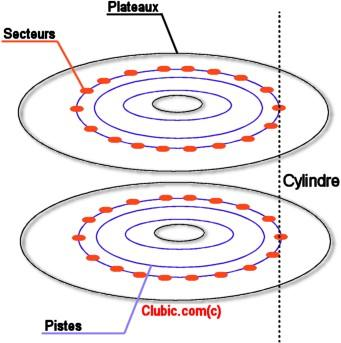
\includegraphics[scale=0.5]{disque_dur.jpg}
    \end{figure}

\end{frame}

%------------------------------------------------------------------------------
% rom5
%------------------------------------------------------------------------------
\begin{frame}{ROM (5)}
    \subt{MBR vs GPT}

    \vspace{15pt}
    {\textbf{Master Boot Record}} : table de partitions + bootloader sur le
    premier secteur 0/0/1 d'un disque dur. Utilisé par le BIOS.

    \vspace{15pt}
    Le MBR limite le nombre de partitions (4) ainsi que leur taille (2.2 To).

    \onslide<2->
    {
        \vspace{15pt}
        Une carte mère avec UEFI (remplaçant du BIOS) ne peut démarrer que sur un
        disque utilisant le système de partitionnement {\textbf{GPT}}. Ce dernier
        remplace le MBR : 128 partitions, 256 To par partition.
    }
\end{frame}

%------------------------------------------------------------------------------
% rom6
%------------------------------------------------------------------------------
\begin{frame}{ROM (6)}
    \subt{Partition}

    \vspace{15pt}
    Fraction d'un disque dur possédant son propre système de fichiers.

    \onslide<2->
    {
        \vspace{15pt}
        \begin{figure}
            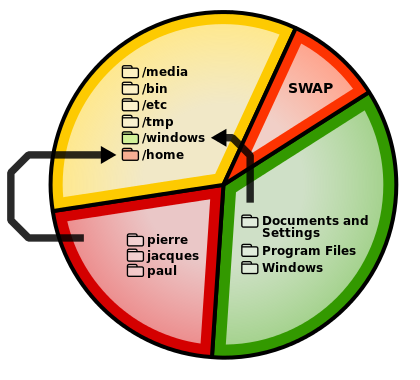
\includegraphics[scale=0.4]{partition.png}
        \end{figure}
    }
\end{frame}

%------------------------------------------------------------------------------
% flash1
%------------------------------------------------------------------------------
\begin{frame}{Flash (1)}
    \subt{Caractéristiques}

    \vspace{8pt}
    EEPROM améliorée : temps de reprogrammation éclair, grosse capacité,
    pas cher!

    \onslide<2->
    {
        \vspace{8pt}
        Lorsque ces mémoires sont intégrées dans des périphériques (comme
        CompactFlash ou SSD), Linux les gère comme des périphériques blocs
        classiques (SATA, USB, ...).

        \vspace{5pt}
        \begin{figure}
            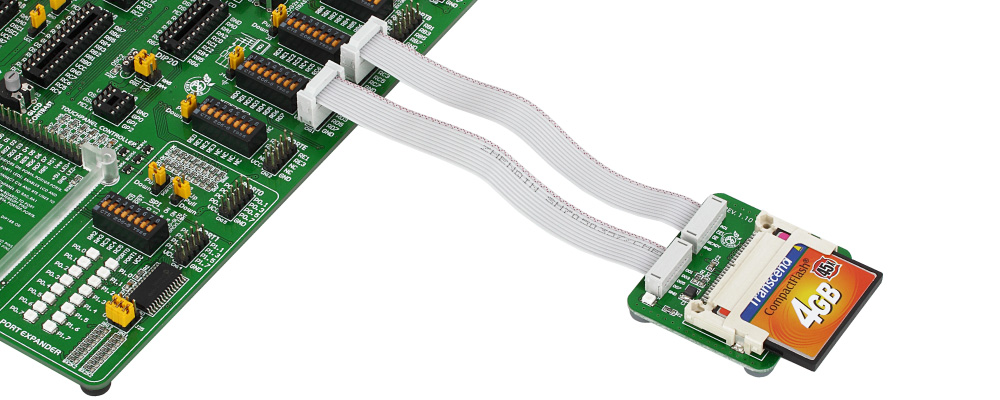
\includegraphics[scale=0.25]{compact_flash.jpg}
        \end{figure}
    }

\end{frame}

%------------------------------------------------------------------------------
% flash2
%------------------------------------------------------------------------------
\begin{frame}{Flash (2)}
    \subt{Partition virtuelle}

    \vspace{8pt}
    Dans les systèmes embarqués, la mémoire flash est souvent intégrée sur les
    cartes mères. \\
    \vspace{8pt}
    => le pilote MTD (Memory Technology Device) est utilisé

    \onslide<2->
    {
        \vspace{8pt}
        Contrairement aux mémoires de masse {\textit{classiques}}, on travaille
        directement avec les adresses mémoires.
    }

    \onslide<3->
    {
        \vspace{5pt}
        \begin{figure}
            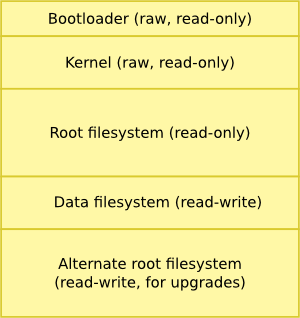
\includegraphics[scale=0.3]{flash-partitions.png}
        \end{figure}
    }

\end{frame}

%------------------------------------------------------------------------------
% flash3
%------------------------------------------------------------------------------
\defverbatim{\lstprocmtd}
{
    \begin{lstlisting}
> cat /proc/mtd
dev:    size   erasesize  name
mtd0: 00300000 00020000 "u-boot"
mtd1: 00080000 00020000 "env"
mtd2: 00080000 00020000 "env2"
mtd3: 00080000 00020000 "dtb"
mtd4: 00080000 00020000 "splash"
mtd5: 00800000 00020000 "kernel"
mtd6: 1c200000 00020000 "rootfs"
mtd7: 03200000 00020000 "user"
    \end{lstlisting}
}

\begin{frame}{Flash (3)}
    \subt{/proc/mtd}

    \vspace{15pt}
    Pour une carte armadeus APF28 :
    \vspace{10pt}
    \lstprocmtd
\end{frame}

%------------------------------------------------------------------------------
% flash4
%------------------------------------------------------------------------------
\begin{frame}{Flash (4)}
    \subt{XIP}

    \vspace{15pt}
    {\textbf{eXecute In Place}} : la mémoire flash de type NOR permet
    d'exécuter du code directement en mémoire sans le charger en RAM.

    \onslide<2->
    {
        \begin{figure}
            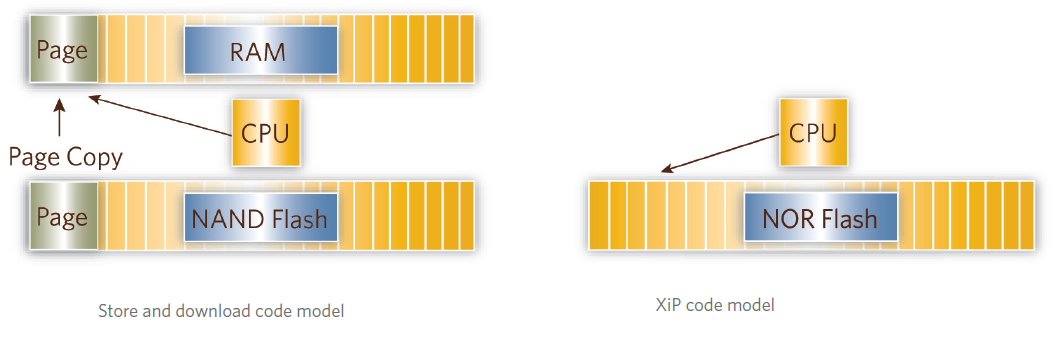
\includegraphics[scale=0.35]{xip.png}
        \end{figure}
    }

    \onslide<3->
    {
        \vspace{10pt}
        De nos jours, la mémoire NAND est la plus utilisée (moins chère)
    }
\end{frame}

%------------------------------------------------------------------------------
% fs1
%------------------------------------------------------------------------------
\begin{frame}{Systèmes de fichiers}
    \subt{Une grande famille...}

    \vspace{15pt}
    Les différents systèmes de fichiers :
    \bi
    \itemsep8pt
    \item {\textbf{VFAT}} : supporté par tous les OS. 4 GB max pour un fichier.
    \item {\textbf{NTFS}} : issu du monde Windows mais supporté sous Linux
          grâce au paquet ntfs-3g.
    \item {\textbf{XFS}} : très efficace pour les I/O parallèles.
    \item {\textbf{EXT2/3/4}} : issu du monde Linux. Vise à remplacer MINIX fs.
    \item {\textbf{JFFS1/2}} : pour les mémoires flash.
    \item {\textbf{UBIFS}} : remplaçant du JFFS2 . Utilise la couche UBI du
          kernel Linux.
    \ei
\end{frame}

%------------------------------------------------------------------------------
% tool1
%------------------------------------------------------------------------------
\begin{frame}{Outils sous Linux (1)}
    \subt{Liste non exhaustive}

    \vspace{10pt}
    \bi
    \itemsep10pt
    \item {\textbf{df}} : report file system disk space usage
    \item {\textbf{blkid}} : locate/print block device attributes
    \item {\textbf{mount/umount}} : mount/unmout a filesystem
    \item {\textbf{fdisk}} : manipulate disk partition table
    \item {\textbf{parted/gparted}} : a partition manipulation program/GUI
    \item {\textbf{mkfs.fat/mkfs.ext2/...}} : build a Linux filesystem
    \item {\textbf{lsblk}} : list block devices
    \ei

\end{frame}

%------------------------------------------------------------------------------
% ftab1
%------------------------------------------------------------------------------
\defverbatim{\lstfstab}
{
    \begin{lstlisting}
> cat /etc/fstab
# /etc/fstab: static file system information.
#
# <fs> <mount point>  <type> <opt> <dump> <pass>
# / was on /dev/sda7 during installation
UUID=XXX-XXX / ext4 errors=remount-ro 0 1
# swap was on /dev/sda5 during installation
UUID=XXX-XXX none swap sw 0 0
/dev/sda2 /media/windows ntfs
/dev/sda6 /media/data ntfs
    \end{lstlisting}
}

\begin{frame}{fstab}
    \subt{Utilité}

    \vspace{15pt}
    {\textbf{fstab}} : liste des disques utilisés ainsi que leurs
    caractéristiques.

    \onslide<2->
    {
        \vspace{15pt}
        \lstfstab
    }
\end{frame}

%------------------------------------------------------------------------------
% concl1
%------------------------------------------------------------------------------
\begin{frame}{Conclusion}

    \centering
    \vspace{20pt}
    \LARGE{
        Dans les sytèmes embarqués, la gestion de la mémoire est un point
        critique!

        \begin{figure}
            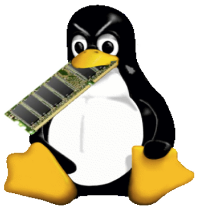
\includegraphics[scale=0.5]{tux_ram.png}
        \end{figure}
    }

\end{frame}

%------------------------------------------------------------------------------
% ref
%------------------------------------------------------------------------------
\begin{frame}{Références}
    \vspace{30pt}

    \bi
    \itemsep12pt
    \item Linux Embarqué - Pierre Ficheux
    \ei

\end{frame}
%<//lecture_content>

\end{document}
